% EJC papers *must* begin with the following two lines. 
\documentclass[12pt]{article}
\usepackage{e-jc}

% Please remove all other commands that change parameters such as
% margins or pagesizes.

% only use standard LaTeX packages
% only include packages that you actually need

% we recommend these ams packages
\usepackage{amsthm,amsmath,amssymb}
\usepackage{verbatim}

% we recommend the graphicx package for importing figures
\usepackage{graphicx}

% use this command to create hyperlinks (optional and recommended)
\usepackage[colorlinks=true,citecolor=black,linkcolor=black,urlcolor=blue]{hyperref}

% use these commands for typesetting doi and arXiv references in the bibliography
\newcommand{\doi}[1]{\href{http://dx.doi.org/#1}{\texttt{doi:#1}}}
\newcommand{\arxiv}[1]{\href{http://arxiv.org/abs/#1}{\texttt{arXiv:#1}}}

% all overfull boxes must be fixed; 
% i.e. there must be no text protruding into the margins


% declare theorem-like environments
\theoremstyle{plain}
\newtheorem{theorem}{Theorem}
\newtheorem{lemma}[theorem]{Lemma}
\newtheorem{corollary}[theorem]{Corollary}
\newtheorem{proposition}[theorem]{Proposition}
\newtheorem{fact}[theorem]{Fact}
\newtheorem{observation}[theorem]{Observation}
\newtheorem{claim}[theorem]{Claim}

\theoremstyle{definition}
\newtheorem{definition}[theorem]{Definition}
\newtheorem{example}[theorem]{Example}
\newtheorem{conjecture}[theorem]{Conjecture}
\newtheorem{open}[theorem]{Open Problem}
\newtheorem{problem}[theorem]{Problem}
\newtheorem{question}[theorem]{Question}

\theoremstyle{remark}
\newtheorem{remark}[theorem]{Remark}
\newtheorem{note}[theorem]{Note}
\newcommand{\F}{\mathcal{F}}
\newcommand{\A}{\mathcal{A}}
\newcommand{\B}{\mathcal{B}}

%%%%%%%%%%%%%%%%%%%%%%%%%%%%%%%%%%%%%%%%%%%%%%%%%%%%%%%

% if needed include a line break (\\) at an appropriate place in the title

\title{\bf An Extension of a Result of Das-Gan-Sudakov}

% input author, affilliation, address and support information as follows;
% the address should include the country, and does not have to include
% the street address 

\author{Erik Waingarten\\
\small Department of Mathematics\\[-0.8ex]
\small Massachusetts Institute of Technology\\[-0.8ex] 
\small Cambridge, MA\\
\small\tt eaw@mit.edu\\
\and
Fermi Ma\\
\small Department of Mathematics\\[-0.8ex]
\small Massachusetts Institute of Technology\\[-0.8ex]
\small Cambridge, MA\\
\small\tt fermima@mit.edu
}

% \date{\dateline{submission date}{acceptance date}\\
% \small Mathematics Subject Classifications: comma separated list of
% MSC codes available from http://www.ams.org/mathscinet/freeTools.html}

\date{\dateline{August, 2014}{XX}\\
\small Mathematics Subject Classifications: XX}

\begin{document}

\maketitle

% E-JC papers must include an abstract. The abstract should consist of a
% succinct statement of background followed by a listing of the
% principal new results that are to be found in the paper. The abstract
% should be informative, clear, and as complete as possible. Phrases
% like "we investigate..." or "we study..." should be kept to a minimum
% in favor of "we prove that..."  or "we show that...".  Do not
% include equation numbers, unexpanded citations (such as "[23]"), or
% any other references to things in the paper that are not defined in
% the abstract. The abstract will be distributed without the rest of the
% paper so it must be entirely self-contained.

\begin{abstract}
Let $B_n$ be the poset of subsets of $[n]$ ordered by inclusion. Given a family $\F$ of elements of $B_n$, a 2-chain is a pair $F_1, F_2 \in \F$ such that $F_1 \subset F_2$. Sperner's theorem states that the largest antichain (a subset with no 2-chains), is exactly the middle ``level" -- all subsets of size $\lfloor \frac{n}{2} \rfloor$. Stanley generalized this result for posets of the form $B_n/G$ where $G$ is a subgroup of the symmetric group $S_n$. Kleitman considered the related problem of minimizing the number of 2-chains for famlies of sets larger than the middle level of $B_n$, and gave a simple algorithm for constructing these families. We generalize this algorithm to $B_n/C_2$ and show via a counterexample that its generalization does not hold for $B_n/G$ with arbritrary $G$.

  % keywords are optional
  \bigskip\noindent \textbf{Keywords:} Sperner's Theorem; Group Actions\end{abstract}

\section{Introduction}

Let $B_n$ be the Boolean lattice, which is the poset of all subsets of $[n]$ with the relation given by set inclusion. Sperner's Theorem is a famous result in combinatorics concerning the size of maximum antichains in $B_n$. For the sake of generalization, we refer to antichains as sets containing no 2-chains, which are pairs $F_1, F_2$ such that $F_1 \subset F_2$. The theorem states states that any family of $B_n$ with no 2-chains has at most $\binom{n}{\lfloor n/2 \rfloor}$ elements, a bound that can be shown to be tight by considering all the subsets of $[n]$ with size $\lfloor n/2 \rfloor$.

We will consider subgroups $G$ of the symmetric group $S_n$ and their corresponding group actions; in particular, we say that two elements $x, y$ of a set $S$ are in the same orbit of $\pi(x) = y$ for some $\pi \in G$. Thus, $G$ partitions sets $S$ into disjoint, nonempty subsets, and we denote by $S / G$ the set of all $G$-orbits of $S$. We will focus on the poset $B_n / G$, where $x < y$ if there exists an element in $x$'s orbit which is a subset of an element in $y$'s orbit. Stanley considered the problem of finding maximum antichains in $B_n / G$, and found that Sperner's Theorem generalizes neatly: the size of the largest antichain is still the size of the largest (and middle) level of the poset.

Kleitman considered the related question of determining the minimum number of a 2-chains that must appear in a family of sets larger than $\binom{n}{\lfloor n/2 \rfloor}$. Das, Gan, and Sudakov considered this problem independently, and extended the result by completely characterizing all extremal families. 

In this paper, we consider an intersection of these two fields of inquiry. We find that the result of Das, Gan, and Sudakov extends to groups of the form $B_n / G$ when $G$ is generated by a single transposition. However, we will show that the same result does not extend to all groups of the form $B_n / G$, as we present a counterexample for a more complicated group $G$. 

\subsection{Additional Notation}

Let the $l$th \emph{level} of $B_n$ or $B_n / G$ refer to all the elements of cardinality $l$.

Definte the $\ell$-shadow of a family by $\partial^{\ell}\F = \{G: \exists F \in \F, G \in F, |G| = |F| - \ell\}$. This notation is due to [Das].

We define $U^i(S)$ for $S \in B_n$ to be the set of supersets of $S$ in $B_n$ with exactly $|S| + i$ elements.

We also define an ordering on all the elements in $B_n$ or $B_n/ G$. Order the levels so that the middle level comes first, followed by the level above, then the level below the middle, then the level above, etc. Within each level, order the elements arbitrarily. We let $l_r$ be the first $r$ elements in this ordering. 


%%%%%%%%%%%%%%%%%%%%%%%%%%%%%%%%%%%%%%%%%%%%%%%%%%%%%%%
\section{Groups Generated By a Transposition}

In this section, we focus on posets of the from $B_n/ G$ where $G$ is generated by a single transposition. Without loss of generality, let this transposition be $(12)$, and denote the group by $G_{(12)}$. 

The $i$th level of $B_n / G_{(12)}$ has size $\binom{n-2}{i-2} + \binom{n-1}{i}$; the first term counts the number of sets that include both 1 and 2, while the second term counts the sets where at most one element of $\{1,2\}$ is included. Since $B_n / G$ is rank-symmetric and unimodal, the largest level consists of elements of size $\lfloor n/2 \rfloor$ and thus has $\binom{n-2}{\lfloor n/2 \rfloor -2} + \binom{n-1}{\lfloor n/2 \rfloor}$ elements. This is the size of the largest family containing no 2-chains [Stanley], and we refer to this quantity as $m$.

Theorem 1.2 of [Das] completely characterizes the minimum number of 2-chains in families $\F$ of subsets of $B_n$. We present a similar result, considering families larger than $m$. 

The following Lemma is due to [Das]. We restate it here for clarity, but an interested reader can find the full proof in [Das].

\begin{lemma}
\label{lemma2}
Let $G$ be a bipartite graph on $U \cup V$ with minimum degree $\delta_U \geq 1$ in $U$ and maximum degree $\Delta_V$ in $V$. Suppose there is no matching from $U$ to $V$. Then there exist nonempty subsets $U_1 \subset U$ and $V_1 \subset V$ with a perfect matching $M: U_1 \to V_1$ and $e(U_1,V) + e(U \setminus U_1,V_1) \leq |U_1| \Delta_V$.
\end{lemma}

The following proposition gives a way to transform a family of sets minimizing the number of 2-chains into another family of sets minimizing the number of 2-chains. 

\begin{proposition}
\label{proposition1} For any $s > m$, there exists a family $\F$ of $s$ elements of $B_n / G_{(12)}$ that minimizes the number of 2-chains and is such that if $A \in \F$ is of maximal cardinality, where we write $|A| = \frac{n}{2}+r$, then for any $B \subset A$ with $|B| \geq \frac{n}{2} - r + 1$, $B \in \F$.
\end{proposition}

\begin{proof} 
Suppose we have a family $\F$ of size $s$ not satisfying this property. Define $\Phi = |\A| + r(m+1)$. We give a procedure by which $\F$ is modified so that it satisfies the desired properties, or $\Phi$ is decreased by at least 1. Since $\Phi \geq 0$, this procedure can be repeated to guarantee that eventually we have a family with the desired properties, which completes the proof.

Let $l \leq 2r-1$ be the smallest integer such that there exists a maximal cardinality set $A \in \F$ with a subset $l$ levels below that is not in $\F$. As in [Das], we define
\begin{align*}
\A &= \{A \in F| \lvert a \rvert = \frac{n}{2}+m, \partial^l A \not\subset \F \}\\
\B &= \partial^l A - \F
\end{align*}

We construct a bipartite graph $G$ on $\A \cup \B$ with an edge $(A,B)$ where $A \in \A$ and $B \in \B$ iff $B \subset A$.

First, consider the case where there exists an injective mapping $M: \A \to \B$. We will show that shifting elements from $\A$ to their corresponding matched elements in $\B$ will shift the elements without increasing the number of 2-chains. Note that if $C \subset B$ for some $B \in \B$ is a 2-chain introduced by the shifting, then $C \subset B \subset A$, so there is no net change in the number of 2-chains. Therefore, it is sufficient to only consider 2-chains added and removed between the levels $\frac{n}{2} + r$ and $\frac{n}{2} + r - l$ (the levels of $\A$ and $\B$, respectively). We will refer to these 2-chains as \emph{intermediate} 2-chains.

Suppose $l > 1$. We will count the number of intermediate 2-chains that we lose and gain from the shifting process in order to show that we lose at least as many 2-chains as we gain.

Because of the minimality of $l$, note that all the $i$-shadows of $\A$ where $1 \leq i \leq l - 1$ must be contained in $\F$. Thus, the number of intermediate 2-chains in $\F$ that we lose is
\[ \sum_{A \in \A}\sum_{i = 1}^{l-1} |\partial^i A | \]
as there exists a 2-chain for every possible pairing of any member of any $i$-shadow of $\A$ (where $1 \leq i \leq l-1$) and any element of $\A$. 

Also, any set in the newly shifted family with cardinality $\frac{n}{2} + r$ must be such that its i-shadows for $1 \leq i \leq l$ are contained in $\F$ (otherwise, this set would have been in $\A$). Thus, we only gain 2-chains from the levels $\frac{n}{2} + r - l$ to $\frac{n}{2} + r - 1$. Then the number of 2-chains that we gain is at most
\[\sum_{A\in \A}\sum_{i = 1}^{l-1} |U^i(M(A)) \cap \F| \]

%perhaps explain the above expression a bit more?

It remains to prove the following Lemma.

\begin{lemma} For any set $\F$ that does not satisfy the properties in Proposition~\ref{proposition1} and is such that there exists an injective matching $M$ from $\A$ to $\B$,
\label{lemma1}
\[ \sum_{A\in \A}\sum_{i = 1}^{l-1} |U^i(M(A)) \cap \F| \leq \sum_{A \in \A}\sum_{i = 1}^{l-1} |\partial^i A | \]
when $l \leq 2r-1$
\end{lemma}

\begin{proof} We first compute $\sum_{A \in \A}\sum_{i = 1}^{l-1} |\partial^i A |$ by considering two cases for $A$.

\textbf{Case 1:} $\{1,2\} \not\subset A$. In this case, each way to select $i$ elements from $A$ corresponds to a distinct member of $\partial^i A$. Thus,
\[ \sum_{i=1}^{l-1} |\partial^i A| = \sum_{i=1}^{l-1}\binom{\frac{n}{2}+r}{i} \]

\textbf{Case 2:} $\{1,2\} \subset A$. This case is different because removing 1 from $A$ gives the same set as removing 2 from $A$. As before, we count the number of ways to select elements to remove so that we count all members of $\partial^i A$.

If we assume that both 1 and 2 are removed, there are $\binom{\frac{n}{2} + r - 2}{i-2}$ ways to pick the other $i-2$ elements. Otherwise, there are $\binom{\frac{n}{2}+r-1}{i}$ ways to pick the $i$ elements to remove, where the $\frac{n}{2} + r - 1$ comes from the fact that selecting 1 is the same as selecting 2. Thus, 
\[ \sum_{i=1}^{l-1} |\partial^i A| = \sum_{i=1}^{l-1} \left( \dbinom{\frac{n}{2}+r-2}{i-2} + \dbinom{\frac{n}{2} + r - 1}{i}\right)\]

Thus, the expression on the right-hand side is equal to
\[ \sum_{\{A | \{1, 2\} \not\subset A, A \in \A\}} \sum_{i=1}^{l-1} \dbinom{\frac{n}{2} + r}{i} + \sum_{\{A | \{1, 2\} \not\subset A, A \in \A\}} \sum_{i=1}^{l-1} \left( \dbinom{\frac{n}{2}+r-1}{i} + \dbinom{\frac{n}{2}+r-2}{i-2}\right) \]

The computation for the left-hand side is similar. We get an upper bound on the size of $|U^i(M(A)) \cap \F|$ by computing the the size of $U^i(M(A))$. We count ways to pick elements from $[n] \setminus M(A)$, the complement of $A$. Since each set in $M(A)$ has $\frac{n}{2} + r - l$ elements, the complement has $\frac{n}{2} - r + l$ elements. 

\textbf{Case 1:} At least one element of $\{1,2\}$ is in $M(A)$. Each way to select $i$ elements from the complement of $M(A)$ correpsonds to a distinct member of $U^i(M(A))$. Thus,
\[ \sum_{i = 1}^{l-1} |U^i(M(A)) \cap \F| \leq \sum_{i=1}^{l-1}\binom{\frac{n}{2}-r+l}{i}\]

\textbf{Case 2:} Neither 1 nor 2 are in $M(A)$. If we assume that both 1 and 2 are added, then there are $\binom{\frac{n}{2}-r + l - 2}{i -2}$ ways to pick the other $i - 2$ elements to add. Otherwise, there are $\binom{\frac{n}{2} - r + l - 1}{i}$ways to pick the $i$ elements to add.

Thus, the expression on the left-hand side is bounded above by
\[ \sum_{\{M(A) | 1 \in M(A) \text{ or } 2 \in M(A)\}} \sum_{i=1}^{l-1} \dbinom{\frac{n}{2}-r+l}{i} + \sum_{\{M(A) | 1, 2 \not\in M(A)\}} \sum_{i=1}^{l-1} \left( \dbinom{\frac{n}{2}-r+l-1}{i} + \dbinom{\frac{n}{2}-r+l-2}{i-2} \right) \]

If we use the fact that $\dbinom{l}{k} > \dbinom{l-1}{k} + \dbinom{l-2}{k-2}$, the left-hand side is bounded above by
\[ |M|\sum_{i=1}^{l-1} \binom{\frac{n}{2}-r+l}{i}\]
where $|M|$ is the size of the matching.
The right-hand side is bounded below by
\[ |M| \sum_{i=1}^{l-1}\left(\binom{\frac{n}{2} + r - 1}{i} + \binom{\frac{n}{2}+r-2}{i-2}\right)\]
Note that
\[ \dbinom{\frac{n}{2}-r+l}{i} \leq \dbinom{\frac{n}{2}+r-1}{i} + \dbinom{\frac{n}{2}+r-2}{i-2} \]
holds when $l \leq 2r-1$. The proof follows.
\end{proof}

Thus, we can perform the shift without gaining any 2-chains. Consider the effect on $\Phi = |\A| + r(m+1)$. If every set in $\A$ has been shifted out for a set in $\B$, then $r$ has decreased by 1 and $\A$ has increased by at most $m$, the size of the maximum level. Otherwise, $r$ has stayed the same but $\A$ has decreased by at least 1. In either case, $\Phi$ decreases.

This leaves the $l = 1$ case. 

%%stopped editing here - fermi

We have at least one missing subset one level below $A$. If there was another set $D \subset A$ where $|D| = |M(A)|$ but $D \in \F$. Then we lose the 2-chain $D \subset A$ and gain no other 2-chains. So we might as well shift all the elements and assume that $\partial \A = \B$. 

So if we shift according to the injective map, we will not increase the number of 2-chains, since the only 2-chains relevant are those between levels of $\A$ and $\B$. If we added a 2-chain, then we had something in level $\frac{n}{2} + r$ that should have been included in $\A$ but was not.

%%started editing again here - fermi

We can recompute $\Phi$ for this new family of sets and see that we have either decreased $r$ by 1 and increased $|\A|$ by at most $m$, or maintained $r$ and decreased $|\A|$ by at least 1. In both cases, $\Phi$ has been decreased by at least 1.

\begin{comment}
%
%
%   I don't see how this is relevant
%
%
First, assume that $r \geq \frac{3}{2}$.
We now show that this means that the sets $A \in \A$ cannot be involved in any 2-chains in $\F$. Once we know that the sets in $\A$ are not involved in any 2-chains, it will allow us to shift them one level down without gaining any 2-chains. Note that if we did increase the number of 2-chains by this switch, it must have been with elements from level $\frac{n}{2}+r$, but these would have been involved in the shift down.

Suppose that there existed a 2-chain with $C \subset A$, and $x \in C$. Then we shift $A$ to $A - \{ x \}$ which is in $\B$ (because $\partial \A = \B$). We also shift the remaining sets in $\A$ by an arbitrary matching from $\A - \{ A \}$ to $\B' = \partial A - \{ A - \{x\} \}$. Note that this matching surely exists by Phillip Hall's Theorem. 

If $X \subset \A - \{ A \}$, then each element in $X$ has at least $\frac{n}{2} + r - 2$ outgoing edges (minus 1 for if it landed on $A - \{x\}$, and minus 1 if 1 and 2 are in the set). Furthermore, each element $B \in \B'$ has at most $\frac{n}{2} - r + 1$ outgoing edges. So if $U \subset X$, and we let $E$ be the number of edges,
\[ |U|*(\frac{n}{2}+r-2) = E \leq (\frac{n}{2}-r+1)|N(U)| \]
So $\dfrac{\frac{n}{2}+r-2}{\frac{n}{2}-r+1} \geq 1$ and since $r \geq \frac{3}{2}$ and in this case we can apply Phillip Hall's Theorem. 
\end{comment}

\begin{comment}
%
%
% I think this is irrelevant now too.
%
%
When $r =1$, the same shift strategy works. Suppose $|\B| = k$. So when we shift out the elements in $\A$, we lose at least $k(\frac{n}{2}) - E(M)$ 2-chains, where $E(M)$ is the total number of edges between all the sets included in the matching. The $\frac{n}{2}$ comes from the fact that for each element in $\A$, it is involved in at least $\frac{n}{2}$ 2-chains (not yet accounting for overcounting). When we shift in the elements from $\B$, we gain at most $k(\frac{n}{2}) - E(M)$ 2-chains, since for each element shifted in, it can be involed in at most $\frac{n}{2}$ 2-chains, and we must subtract $E(M)$ to account for overcounting.

In the shifted set, we have lost the 2-chain $C \subset A$ and gained no intermediate 2-chains. So the shifted set has fewer 2-chains. Therefore, the sets in $\A$ cannot be part of any 2-chains. So the shifted set to $\partial \A$ will not be in any 2-chains. 
\end{comment}

\begin{comment}
%
%
%   I don't think this is relevant.
%
%
Since $|\F|$ is greater than the middle level, we know that there is some 2-chain, suppose it is $C \subset D$. So we can additionally shift $D$ to some element in $\partial \A$. We know there is an available since $|\partial \A| > |\A|$ for $r \geq 1$. This is because each set $A \in \A$ has at least $\frac{n}{2}+r-1$ outgoing edges and each $B \in \partial \A$ has at most $\frac{n}{2}-r+1$ outgoing edges; similarly to before, $\dfrac{\frac{n}{2}+r-1}{\frac{n}{2}-r+1} > 1$ when $r \geq \frac{3}{2}$. 
\end{comment}

Now we assume there does not exist an injective map from $\A \rightarrow \B$.

We apply Lemma~\ref{lemma2} to the bipartite graph on $\A \cup \B$, as we satisfy the conditions of the lemma with $U = \A, V = \B, \Delta_V = \dbinom{\frac{n}{2} - r + l}{l}$.

The lemma produces $\A_1 \subset \A$, $\B_1 \subset \B$, and a matching $M:\A_1 \rightarrow \B_1$. We shift the elements from $\A_1$ to $B_1$, and since $M(A) \subset A$, we only need to consider intermediate 2-chains. Since $r \geq 1$, the same calculation used in the proof of Lemma~\ref{lemma1} shows that the number of 2-chains decreases. Thus, we only need to consider the 2-chains destroyed and created between $\A$ and $\B$, or levels $\frac{n}{2} + r$ and $\frac{n}{2} + r - l$.

%should we say instead that the number of 2-chains does not increase? in the paragraph above. Also should the sentence about only considering intermediate 2-chains be moved to the end of the paragraph? the last sentence is essentially saying that we're only considering intermediate 2-chains...

The number of 2-chains created by the shifting is $e(\A - \A_1, \B_1)$. We lose the 2-chains between $\A_1$ and $\partial^l\A_1 \cap \F = \partial^l\A_1 - \B$, which is at least
\[ |\A_1|\dbinom{\frac{n}{2}+r-1}{l} - e(\A_1, \B) \geq |\A_1|\dbinom{\frac{n}{2} - r + l}{l} - e(\A_1, \B) \geq e(\A - \A_1, \B_1) \] 
Therefore, we can perform the shift without a net gain in 2-chains.

If we compute $\Phi$, we see that although $r$ stayed the same, $|\A|$ has decreased by at least 1.
\end{proof}


%%stopped editing here - fermi 
\begin{corollary}
\label{cor1}
There exists a family of $s > m$ subsets satisfying the properties in Proposition~\ref{proposition1} and is such that if $A \in \F$ is of minimal cardinality, where we write $|A|=\frac{n}{2}-r$, then for any $A \subset B$ with $|B| \leq \frac{n}{2}+r-1$, $B \in \F$
\end{corollary}

\begin{proof}
Once we have a family satisfying Proposition~\ref{proposition1}, we can take complements and apply the same transformation as in the proof of Proposition~\ref{proposition1}.
\end{proof}

\begin{proposition}
\label{proposition2}
Suppose we have a family of sets satisfying the properties of Corollary~\ref{cor1} and with elements lying between levels $\frac{n}{2}\pm r$, then we can always move elements from the level $\frac{n}{2} \pm r$ into a middle level ($\frac{n}{2} + r - l$, where $1 \leq l \leq 2r-1$) without adding more 2-chains. 
\end{proposition}

\begin{proof}
Lets just shift an element from the $\frac{n}{2} + r$ level into a middle level and count the number of 2-chains added and subtracted. 

By removing the top level element, we have removed at least
\[ \sum_{i=1}^{2r-1} \left(\dbinom{\frac{n}{2} +r-1}{i} + \dbinom{\frac{n}{2} + r-2}{i-2}\right) \]
and have added at most
\[ \sum_{i=1}^{l-1}\dbinom{\frac{n}{2}-r + l}{i} + \sum_{i=1}^{2r-l} \dbinom{\frac{n}{2}+r-l}{i} \]
Note that we couldn't have added elements on top since by property 1, they were not included.

We upper bound terms of the form $\binom{\frac{n}{2}+r-l}{i}$ with $\binom{\frac{n}{2}+r-1}{i}$, so the net total reduction in 2-chains is at least
\[ \sum_{i=1}^{2r-1} \dbinom{\frac{n}{2}+r-2}{i-2} + \sum_{i=2r-l+1}^{2r-1} \dbinom{\frac{n}{2}+r-1}{i} - \sum_{i=1}^{l-1} \dbinom{\frac{n}{2}-r+l}{i}\]
\[ \geq \sum_{i=1}^{l-1} \left(\dbinom{\frac{n}{2}+r-1}{2r-i} - \dbinom{\frac{n}{2}-r+l}{i}\right) \]
\[ \geq \sum_{i=1}^{l-1} \left(\dbinom{\frac{n}{2}+r-1}{\frac{n}{2}-r-1+i} - \dbinom{\frac{n}{2}+r-1}{i}\right) \geq 0 \]
To see this, it is easy to see that the sum of the first $l-1$ binomial coefficients will be at most the sum of the $l-1$ binomial coefficients starting at the $i$th coefficient.

Therefore, we can always move the elements from level $\frac{n}{2}+r$ to some missing spots in the middle without adding 2-chains. 
\end{proof}

\begin{theorem} For any $s \geq m$, let $r \in \frac{1}{2}\mathbb{N}$ be the unique half-integer such that $\sum_{i = \frac{n}{2} - r +1}^{\frac{n}{2} + r -1} |P_i| < s \leq \sum_{i = \frac{n}{2}-r}^{\frac{n}{2}+r}|P_i|$. There exists a family of subsets $\F$ of $B_n / G_{(12)}$ with $|\F| = s$ minimizing the number of 2-chains satisfying the following properties:

1) For every $A \in \F$, $n/2 - r \leq |A| \leq n/2 + r$

2) For any $A \in B_n / G_{(12)}$ with $n/2 - r + 1 \leq |A| \leq n/2 + r - 1$, we have $A \in \F$.
\end{theorem}

\begin{proof}
We prove this with induction on $s$.

For the base case, $s = m$. If $n$ is even and $r = 0$, then $\F$ only has elements from the middle level and [Stanley] tells us that this is minimizing the number of 2-chains. If $n$ is odd and $r = \frac{1}{2}$, then $\F$ has elements from the middle two levels. Property 2 does not mean anything. [Stanley] tells us that these families minimize the number of 2-chains. 

For the inductive step, take a family of sets $\F_0$ with $s-1$ elements that satisfies the properties and minimizes the number of 2-chains for $s-1$ elements. First, we analyze the case where the $\frac{n}{2}+r$ level is not full, so we add a set $F_0$ to the level $\frac{n}{2} + r$. Note that $\F_0 \cup \{F_0\}$ still satisfies properties 1 through 4.

We will assume that there exists a different family with fewer 2-chains and show that if one of the properties is broken, there isn't less 2-chains than in $\F_0 \cup \{ F_0\}$. Therefore, this will show that there exists a family of sets which satisfies the above properties and minimzes the number of 2-chains.

We separate the claim into two cases:

\begin{itemize}
\item Case 1: $\{1, 2\} \subset F_0$.
\item Case 2: $\{ 1, 2\} \not\subset F_0$.
\end{itemize}

Now suppose a family $\F$ of $s > m$ sets satisfying the conditions of Propostion~\ref{proposition1} has fewer 2-chains than $\F_0 \cup \{F_0\}$. Suppose this family does not satisfy Property 1. Since $\F$ and $\F' = \{ [n] - F | F \in \F \}$ are involved in the same number of 2-chains, we can assume that the largest element $F \in \F$ has $|F| = \frac{n}{2} + t$ where $t > r$. 

Then from Proposition~\ref{proposition1}, we know that every $G \subset F$, where $|G| \geq \frac{n}{2}-t+1$, we have $G \in \F$. So $F$ is involved in at least
\[ \sum_{i=1}^{2t-1} \dbinom{\frac{n}{2}+t - 1}{i} + \dbinom{\frac{n}{2}+t-2}{i-2}\]
2-chains. So there are at least $c_2(n, s-1) + \sum_{i=1}^{2t-1} \dbinom{\frac{n}{2}+t - 1}{i} + \dbinom{\frac{n}{2}+t-2}{i-2}$ 2-chains in $\F$, but since we assumed that $\F_0$ was optimal for $s-1$ elements, we know that $\F_0 \cup \{F_0\}$ has at most
\[ c_2(n, s-1) + \sum_{i=1}^{2r-1} \dbinom{\frac{n}{2}+r - 1}{i} + \dbinom{\frac{n}{2}+r-2}{i-2} \]
2-chains since the $\frac{n}{2}-r$ level is empty and we are dealing with Case 1. Since $t > r$, we know that $\F$ has more 2-chains than $\F_0$, which means that $\F$ must satisfy Property 1.

So now suppose $\F$ satisfies property 1 but not property 2. Then in light of property 1, we know that $\F$ has some element in level $\frac{n}{2} \pm r$, and again by symmetry, we can assume that it is in level $\frac{n}{2} + r$ by taking complements. Therefore, we know that $\F$ is involved in at least 
\[ c_2(n, s-1) + \sum_{i=1}^{2r-1} \dbinom{\frac{n}{2}+r - 1}{i} + \dbinom{\frac{n}{2}+r-2}{i-2} \]
and thus doesn't have less 2-chains. 

Now we can analyze Case 2, where $\{ 1, 2\} \not\subset F_0$. In this case, if we have family $\F$ with less 2-chains which broke property 1, we would have an element with a set in a level $t > r$ and so $\F$ would have at least
\[ c_2(n, s-1) + \sum_{i=1}^{2t-1} \dbinom{\frac{n}{2}+t-1}{i} + \dbinom{\frac{n}{2}+t-2}{i-2} \]
But we know that $\F_0 \cup \{ F_0\}$ has at most
\[ c_2(n,s-1) + \sum_{i=1}^{2r} \dbinom{\frac{n}{2}+r}{i} \]
which is not more than the number of 2-chains in $\F$ since $t \geq r + 1$. So we get Property 1 in this Case 2 as well. 

Suppose $\F$ satisfied property 1 but not property 2, then we know that there is an element in level $\frac{n}{2} \pm r$ and an element missing inside in level $\frac{n}{2}+r-l$. We can move the elements down via Proposition~\ref{proposition2}. This gives us property 2. 
\end{proof}

%%%%%%%%%%%%%%%%%%%%%%%%%%%%%%%%%%%%%%%%%%%%%%%%%%%%%%%
\section{A Counterexample for a Different $G$}

This result does not extend to $B_n / G$ for any $G$. In particular, let $n = 6$ and let $G$ be the group generated by the transpositions $(12), (23),$ and $(34)$. An the following figure gives an example of a collection of 12 sets that is not taken by the middle levels and has less 2-chains than the collection of the 12 middle sets.
\begin{center}
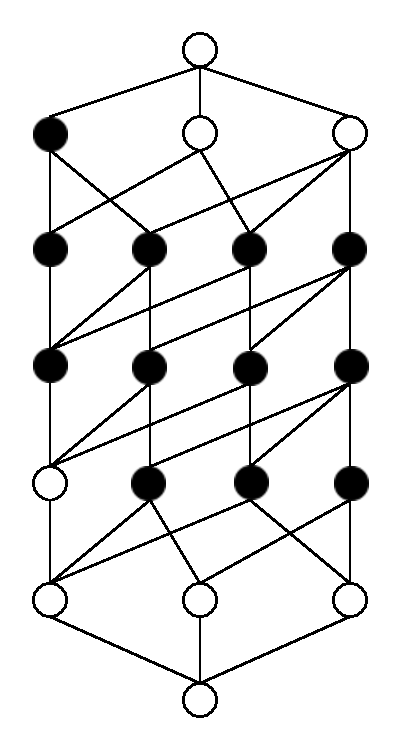
\includegraphics[scale=0.7]{counterexamplegraph.pdf}
\end{center}

%%%%%%%%%%%%%%%%%%%%%%%%%%%%%%%%%%%%%%%%%%%%%%%%%%%%%%%
\section{Conclusion}

%definitely expand this!

We were able to characterize certain families of $B_n / G_{(12)}$ that minimize the number of 2-chains, and we gave an algorithm to construct minimizing families. We showed by providing a simple counterexample that our general characterization of minimizing families does not extend to general $B_n / G$ for arbitrary groups $G$.

Our research leaves a few open questions for further study. In particular, there may be other groups $G$ for which $B_n / G$ behaves similarly to $B_n / G_{(12)}$. 

%%%%%%%%%%%%%%%%%%%%%%%%%%%%%%%%%%%%%%%%%%%%%%%%%%%%%%%
\subsection*{Acknowledgements}
We thank Jonathan Novak (MIT) for guiding our research and providing helpful discussions.

%%%%%%%%%%%%%%%%%%%%%%%%%%%%%%%%%%%%%%%%%%%%%%%%%%%%%%%
% \bibliographystyle{plain} 
% \bibliography{myBibFile} 
% If you use BibTeX to create a bibliography
% then copy and past the contents of your .bbl file into your .tex file

\begin{thebibliography}{10}

\end{thebibliography}

\end{document}
